% ------------------------------------------
%  MASTER THESIS DISSERTATION
% ------------------------------------------
% Author:
%
% Advisors:
%
% ------------------------------------------
\documentclass[10pt,twoside,openright,a4paper]{report}
\usepackage[utf8]{inputenc}

% Set document margins to 1in in all sides
\usepackage[margin=2.5cm]{geometry}
% Line spacing package
\usepackage{graphicx, helvet, hyperref, setspace}
\usepackage[portuguese,english]{babel}
\usepackage[acronym, toc]{glossaries}
% Extra stuff file
% This file is included before begin{document} environment
% Use this to include extra packages and define your own commands
% This way, you can easily grab a most recent version
% of dissertation.tex file from the original repo
\usepackage[table]{xcolor}
\definecolor{HeaderRowColor}{RGB}{101,204,255}
\definecolor{EvenRowColor}{RGB}{210,241,255}
\definecolor{OddRowColor}{RGB}{255,255,255}



\graphicspath{{images/}}
% Built the glossary when the main file is built.
\makeglossaries
% Set main font to Arial
\renewcommand{\familydefault}{\sfdefault}
% Define keywords macro
\providecommand{\keywords}[1]{\textbf{Keywords:} #1}
% Define "palavras-chave" macro
\providecommand{\palavrasChave}[1]{\textbf{Palavras-Chave:} #1}
% Define the NewPage macro
\newcommand*\NewPage{\newpage\null\thispagestyle{empty}\cleardoublepage}
% Abstract-en page numbering
\newcommand {\abstractEnglishPageNumber} {\thispagestyle{plain}\setcounter{page}{\abstractEnglishPage}}
% Abstract-pt page numbering
\newcommand {\abstractPortuguesePageNumber} {\thispagestyle{plain}\setcounter{page}{\abstractPortuguesePage}}
% Section numbering depth
\setcounter{secnumdepth}{2}
% Table of contents depth
\setcounter{tocdepth}{3}
% Set line spacing to 1.5cm
\onehalfspacing
% Page numbering
\pagestyle{plain}

% Glossary-File
% Glossary Definition
\newglossaryentry{MACAddress}{name={MAC Address}, description={The Media Access Control Address is a 48-bit address typically imprinted in the network access hardware that uniquely identifies a device within a local area network scope}}
\newglossaryentry{IPAddress}{name={IP Address}, description={A numeric address globally identifying a device connected to a network running the Internet Protocol}}
\newglossaryentry{Keepalive}{name={Keepalive}, description={A periodic message sent from the station at one end of a communication channel to the station at the other end of the channel in order to check that the channel is still active and keep it active}}
\newglossaryentry{anycast}{name={Anycast},description={A one-to-nearest communication paradigm in which multiple instances of the receiver exist and datagrams sent by a sender are delivered to the nearest receiver.}}
% Acronym-File
% Acronym Definition
\newacronym{SDN}{SDN}{Software-Defined Network}
\newacronym{IDS}{IDS}{Intrusion Detection System}
\newacronym{WAN}{WAN}{Wide Area Network}
\newacronym{IT}{IT}{Information Technology}
\newacronym{VM}{VM}{Virtual Machine}
\newacronym{IaaS}{IaaS}{Infrastructure as a Service}
\newacronym{MPLS}{MPLS}{Multiprotocol Label Switching}
\newacronym{VLAN}{VLAN}{Virtual Local Area Network}
\newacronym{NAT}{NAT}{Network Address Translation}
\newacronym{VRF}{VRF}{Virtual Routing and Forwarding}
\newacronym{NFV}{NFV}{Network Function Virtualization}
\newacronym{ETSI}{ETSI}{European Telecommunications Standards Institute}
\newacronym{API}{API}{Application Programming Interface}
\newacronym{NOS}{NOS}{Network Operating System}
\newacronym{ONF}{ONF}{Open Networking Foundation}
\newacronym{POF}{POF}{Protocol Oblivious Forwarding}
\newacronym{ForCES}{ForCES}{Forwarding and Control Element Separation}
\newacronym{CPU}{CPU}{Central Processing Unit}
\newacronym{IETF}{IETF}{Internet Engineering Task Force}
\newacronym{OVSDB}{OVSDB}{Open vSwitch Database}
\newacronym{OF-CONFIG}{OF-CONFIG}{OpenFlow Management and Configuration Protocol}
\newacronym{TLS}{TLS}{Transport Layer Security}
\newacronym{TCP}{TCP}{Transmission Control Protocol}
\newacronym{QoS}{QoS}{Quality of Service}
\newacronym{MIB}{MIB}{Management Information Base}
\newacronym{LLDP}{LLDP}{Link Layer Discovery Protocol}

% ------------------------------------------
% MASTER THESIS DISSERTATION
% ------------------------------------------

\begin{document}
\pagenumbering{gobble}% Remove page numbers (and reset to 1)
\clearpage
\thispagestyle{empty}
%!TEX root = ./dissertation.tex

% Dissertation basic information
\newcommand {\Title} {A Scalable Architecture for OpenFlow SDN Controllers}
\newcommand {\Subtitle} {}
\newcommand {\StudentName} {Filipe Fernandes Azevedo}
\newcommand {\DegreeName} {Master Degree in Information Systems and Computer Engineering}
\newcommand {\Supervisors} {{\large Prof. Fernando Henrique Côrte-Real Mira da Silva}\\{\large Prof. Luís Jorge Brás Monteiro Guerra e Silva}}

% Include or not include acknowledgments
\def \includeAcknowledgments{1}

% Include or not include glossary
\def \includeGlossary{1}

% Examination Committee
\newcommand {\Advisor} {{\large Prof. Fernando Henrique Côrte-Real Mira da Silva}}
\newcommand {\CoAdvisor} {{\large Prof. Luís Jorge Brás Monteiro Guerra e Silva}}

% After the thesis defense
\newcommand {\CommitteeMembers} {
{\large Prof./Dr. Lorem Ipsum}\\
{\large Prof./Dr. Lorem Ipsum}
}
\newcommand {\Chairperson} {{\large Prof./Dr. Lorem Ipsum}}

% Is final version (will include Committee Members information)
\def \IsFinalVersion{0}

% Date
\newcommand {\Month} {October}
\newcommand {\Year} {2015}

% Acknowledgments page number
\def \acknowledgmentsPage{1}

% Abstract-en page numbering
\def \abstractEnglishPage{3}

% Abstract-pt page number
\def \abstractPortuguesePage{5}

% You had a co-advisor:
\def \HasCoAdvisor{1}

% Logo Spacing Variables
\def \finalLogoSpacing{2.0cm}
\def \draftLogoSpacing{2.0cm}

% Advisors Spacing Variables
\def \finalAdvisorsSpacing{1.0cm}
\def \draftAdvisorsSpacing{8.0cm}

% Date Spacing Variable
\def \dateSpacing{4.0cm}

% You can define your own variables here


%!TEX root = ./dissertation.tex

% ---------------------------------------------------------
%   MASTER THESIS DISSERTATION COVER
% ---------------------------------------------------------
\begin{titlepage}
% ---------------------------------------------------------
%  INSTITUTION LOGO
% ---------------------------------------------------------
\includegraphics[width=5cm]{images/ist_logo}~\\
%
\if\IsFinalVersion 1
  \vspace*{\finalLogoSpacing}
\else
  \vspace*{\draftLogoSpacing}
\fi

\begin{center}
\if\IsFinalVersion 1
\vspace*{1.5cm}
\fi
% ---------------------------------------------------------
%  MASTER THESIS DISSERTATION TITLE
% ---------------------------------------------------------
{\LARGE \textbf{\Title}}\\[1.0cm]
\if\IsFinalVersion 0
\vspace*{0.8cm}
\fi
% ---------------------------------------------------------
%  AUTHOR NAME (FULL)
% ---------------------------------------------------------
\if\IsFinalVersion 1
\vspace*{0.3cm}
\fi
{\Large \textbf{\StudentName}}\\[1.0cm]
\if\IsFinalVersion 1
\vspace*{0.3cm}
\fi
% ---------------------------------------------------------
%  DISSERTATION DEGREE
% -----------------------------------------------------------------
{\large Thesis to obtain the Master of Science Degree in}\\[0.5cm]
% -----------------------------------------------------------------
%  COURSE NAME
% -----------------------------------------------------------------
{\LARGE \textbf{\DegreeName}}\\[1.0cm]
% -----------------------------------------------------------------
%  ADVISORS NAME
% ---------------------------------------------------------
%\begin{minipage}[t]{.5\textwidth}
%  \begin{flushright}
    {\large Supervisors:\:}
%\end{flushright}
%\end{minipage}%
%\begin{minipage}[t]{.5\textwidth}
%  \begin{flushleft}
    {\Supervisors}\\
%  \end{flushleft}
%\end{minipage}\\
%
\if\IsFinalVersion 1
  \vspace*{\finalAdvisorsSpacing}
\else
  \vspace*{\draftAdvisorsSpacing}
\fi
% ---------------------------------------------------------
%  JURI NAMES:
%  - PRESIDENT
%  - ADVISOR
%  - VOGALS
% ---------------------------------------------------------
\if\IsFinalVersion 1
%
\vspace*{1.2cm}
{\Large \textbf{Examination Committee}}\\[.25cm]
%\begin{minipage}[t]{.5\textwidth}
%  \begin{flushright}
    \if\IsFinalVersion 1
    {\large Chairperson:\:}
    {\Chairperson}\\
    \fi
    {\large Supervisor:\:}
    {\Advisor}
%    \hfill \break
    \if\IsFinalVersion 1
    {\large Member of the Committee:\:}
    {\CommitteeMembers}
    \fi
%  \end{flushright}
%\end{minipage}%
%\begin{minipage}[t]{.5\textwidth}
%  \begin{flushleft}
%    \if\IsFinalVersion 1
%    {\Chairperson}\\
%    \fi
%    {\Advisor}
%    \if\IsFinalVersion 1
%    {\CommitteeMembers}
%    \fi
%  \end{flushleft}
%\end{minipage}\\[1.0cm]
%
\fi

\if\IsFinalVersion 1
 \vspace*{\dateSpacing}
\fi

% ---------------------------------------------------------
%  DATE (MONTH AND YEAR)
% ---------------------------------------------------------
{\Large \textbf{\Month\:\Year}}\\
\end{center}
\end{titlepage}

\NewPage

\pagenumbering{roman}

\if\includeAcknowledgments 1
%!TEX root = ../dissertation.tex

% Acknowledgments: This one is optional
\chapter*{Acknowledgments}
I would like to thank every one, from friends and colleagues to family, who in one way or another helped achieve this life goal.\\
There are however a couple of you who have been there all along, helping me raise the bar day by day, namely my parents, Sancho and Susana, to whom I hold deep gratitude for everything they have done throughout my whole life, my girlfriend, Mariana, who was there all along offering unconditional support, my aunts and uncles, Madalena, Júlio, Maurício and Catarina who offered me more than I could ask for and without whom I could not get all the way to where I am, and my dear friend João, who through countless lunch hours put up with my problems and supported me along the way.\\
Last but definitely not least, I would like to express my sincere gratitude to my advisors, Professor Fernando Mira da Silva and Professor Luís Guerra e Silva, for excellent mentorship and all the support given that at times went beyond the role of advisor.
\NewPage
\fi

%!TEX root = ../dissertation.tex

\begin{otherlanguage}{english}
\begin{abstract}
% Set the page style to show the page number
\thispagestyle{plain}
\abstractEnglishPageNumber
% Problem statement
Today's computer network environments are in essence a complex device-centric web, made out of thousands of autonomous devices - network nodes - and connections in between them through which the said nodes communicate with each other by means of communication protocols.
The result is a highly inflexible infrastructure that is hard to manage, maintain and evolve. 
In order to modify the behavior of today's network these nodes have to be manually configured in a vendor specific manner, which renders the introduction of modifications slow, prone to Human error and dependent on the vendor's implementation of the protocols.
The recent server virtualization trend has made the data center a much more dynamic environment by effectively increasing the number of computing instances that have different and changing network requirements, resulting in an increased pressure on data center network management not only for network availability but security and scalability as well, specially when we consider multi-tenant data center environments.\\
% What is SDN & OF
\emph{Software-Defined Networking}, along with its most prominent supporting protocol - \emph{OpenFlow} -, presents itself as a new paradigm capable of solving the aforementioned issues by means of separating the data forwarding logic from the control logic and allowing for a logically centralized, standardized, programmable network management interface.
SDN relies essentially on the decoupling of the \emph{control plane} from the \emph{data plane}, placing the former in a logically centralized component to be executed on commodity hardware - the \emph{SDN Controller}.\\
% How OF works & associated limitations
The OpenFlow protocol features proactive and reactive programming.
The proactive mode is based on static programming of the data plane.
Reactive programming enables the programming of the network based on real-time decisions taken as new traffic hits the data plane, but it requires the first packet of every new flow traversing any SDN controlled network node to be sent to the controller and evaluated.
The proper action is then programmed in the device, and the packet is sent back to the data plane.
While reactive mode offers a much more convenient and flexible method to program the network when compared with proactive mode, the inherent computational cost of performing the associated tasks in large networks becomes too large to be handled by a single SDN Controller instance.
One way to overcome this limitation is to have several SDN Controller instances running separately, each one handling a subset of network devices.
However, this solution requires  a complex and cumbersome configuration of both SDN controllers and OpenFlow devices in order to keep consistent network rules and efficient load sharing across controllers.\\
% Our solution
In order to make the most out of OpenFlow's potential, a new architecture for OpenFlow SDN controllers has been developed, centered on the concept of elastic SDN Controller clustering and anycast communication paradigm.
The proposed architecture offers both load balance between different SDN controller instances and a resilient infrastructure to deal with the loss of any single controller, allowing for a scalable use of reactive flow programming. 
% Keywords
\begin{flushleft}

\keywords{Software-Defined Networking, OpenFlow, Network Function Virtualization, Network Management, Distributed SDN Controller}

\end{flushleft}

\end{abstract}
\end{otherlanguage}

\NewPage
%!TEX root = ../dissertation.tex

\begin{otherlanguage}{portuguese}
\begin{abstract}
\abstractPortuguesePageNumber

% What is SDN & OF
O padrão arquitetural Software-Defined Network \gls{SDN} e o seu protocolo mais proeminente - \emph{OpenFlow} - continuam a ganhar ímpeto.
A arquitetura \gls{SDN} tem por base o desacoplamento do \emph{control plane} do \emph{data plane}, colocando o primeiro num novo componente logicamente centralizado a ser executado em hardware de comodidade - o \emph{Controlador \gls{SDN}}.
% How OF works & associated limitations
O modo de programação reativa do OpenFlow permite a programação da rede em tempo real, tomando decisões de encaminhamento conforme o tráfego dá entrada no \emph{data plane}, sendo necessário para tal que a primeira trama de cada fluxo que atravesse um qualquer dispositivo de rede gerido por um controlador \gls{SDN} seja reencaminhado para o controlador para que seja inspecionado.
Embora o modo reativo proporcione um método mais conveniente e flexível para programar a rede quando comparado com o modo proactivo, o custo computacional associado à execução das tarefas necessárias torna-se incomportável para ser executado por uma única instância do controlador \gls{SDN} quando aplicado a redes de grande dimensão.\\
% My work
Propõe-se neste documento uma nova arquitetura que torna o controlador \gls{SDN} num cluster elástico visando a solução para o problema de escalabilidade apresentado através da existência de várias instâncias de controlador \gls{SDN} que atuam como um único controlador, ficando no entanto cada instância responsável pela gestão de um subconjunto dos switches OpenFlow que compõem a rede.
Houve ainda lugar a uma implementação de prova de conceito através da extensão do controlador Floodlight e da integração com o projeto Linux Virtual Server.
% Keywords
\begin{flushleft}

\keywords{Software-Defined Networking, OpenFlow, Gestão de redes, Controlador \gls{SDN} Distribuído}

\end{flushleft}

\end{abstract}
\end{otherlanguage}

\NewPage

% Table of contents
\tableofcontents
% A new page is necessary only if table of contents has an odd number of pages
\NewPage

% List of tables
\addcontentsline{toc}{chapter}{\listtablename}
\listoftables
% A new page is necessary only if list of tables has an odd number of pages
\NewPage

% List of figures
\addcontentsline{toc}{chapter}{\listfigurename}
\listoffigures
% A new page is necessary only if list of figures has an odd number of pages
\NewPage

% List of acronyms
\printglossary[type=\acronymtype]
\cleardoublepage

\pagenumbering{arabic}% Arabic page numbers (and reset to 1)

%!TEX root = ../dissertation.tex

% Entry point for chapters
% In this file you define the order
% in which the chapters are included

% Chapters
%!TEX root = ../dissertation.tex

\chapter{Introduction}
\label{chapter:introduction}
% Traditional network paradigm & management problem
Today's computer networks are essentially sets of interconnected network nodes. 
These nodes are mainly proprietary black boxes that allow for data input/output, exposing a configuration interface through which network operators can configure its behavior by means of a vendor specific configuration workflow and interface.
These black boxes are typically switches and routers that implement in software and/or hardware a set of standard or proprietary protocols that allow them to communicate with each other and provide service to the endpoints logically or physically connected to them.
Because the process of creating and implementing new protocols requires a long period of time, and due to the complex dependency between multiple protocols running on the same node, new network features have typically been implemented resorting to middle boxes designed to perform specific functions such as Firewalls, \glspl{IDS} and \gls{WAN} optimizers, thus effectively increasing the overall complexity and in turn further aggravating the network manageability issue at hand.\\
%
% IT virtualization adding pressure
This has held true for the last couple of decades and is now an increasingly focus of attentions due to the recent trend of \gls{IT} virtualization trend, that has changed the typical data center environment drastically, with the number of virtual network ports surpassing that of physical network ports and the amount of virtual servers largely exceeding the number of physical servers\cite{Kreutz2014}.
However, \gls{IT} virtualization has a much deeper impact on the data center network infrastructure than the mere increase of network ports and hosts.
With today's \gls{IT} virtualization technology, the creation, removal and relocation of \glspl{VM} between physical hosts are trivial operations thus allowing for the concept of \gls{IaaS} to emerge, which in turn allows for the creation of elastic computing services\cite{Kreutz2014} such as Amazon Elastic Compute Cloud (Amazon EC2)\cite{AmazonEC2}.
The \gls{IT} virtualization operations supporting \gls{IaaS} can be performed in a matter of minutes, however the network infrastructure must be reconfigured as well to support the changes being made to the environment, and it must be done manually and often node by node, taking hours or even days to do so.\\
%
% Existing virtualization solutions & associated problems
Current networking concepts already introduced virtualization mechanisms, such as \gls{MPLS} for path virtualization, \gls{VLAN} for layer 2 virtualization and \gls{NAT} and \gls{VRF} for layer 3 virtualization\cite{Kreutz2014}, however, these solutions are still device-centric and therefore still require configuration to be performed node by node through the same vendor specific workflows and interfaces, meaning that there is still no global network view nor global network configuration\cite{Kreutz2014} and in some cases these mechanisms are no longer able to cope with the high density of compute instances introduced by \gls{IT} virtualization \cite{Duffy2012} thus leaving the task of network reconfiguration to still require a large amount of time, be error prone and in some cases ineffective.
As a result, networks are now the technological bottleneck that is dragging the operational workload and hindering innovation in \gls{IT}, with heavy focus on data center environments.
To that extent a new network management model is now required, one that can cope with the requirements now being set while also being future proof.\\
%
% New generation solutions
In order to solve these issues two new concepts arose in the past couple of years, \glspl{SDN} and \gls{NFV}.
These two concepts share some core concerns, such as the use of commodity hardware to implement network features, but they both aim at different goals, being considered to be complementary but not dependent on each other\cite{ETSI2014}\cite{Pate2013}.\\
%
% NFV
\gls{NFV} was proposed by the \gls{ETSI} and stems from \gls{IT} virtualization itself, proposing the virtualization of entire network node classes, such as Firewalls, Routers and \glspl{IDS}, using commodity hardware as the underlying physical infrastructure.
This concept results in the dismissal of function-specific hardware middle boxes by means of virtualization, thus easing the physical constrains of adding new features to the network, as new instances of virtualized nodes can be deployed using existing commodity hardware already in place in different regions of the network\cite{ETSI2014}.
This means that at core, \gls{NFV} attempts to improve the scalability of current networks by removing some of the hardware complexity and cost but leaves the global network manageability issue yet to be solved.\\
%
% SDN
The current notion of \gls{SDN} was developed in Stanford University while researching for a network configuration protocol, from which resulted OpenFlow, and is a concept that keeps gaining momentum both on the academic and business environments.
\gls{SDN} refers to the architectural principles while OpenFlow is an implementation of a supporting protocol for the said architecture.
\gls{SDN} relies essentially on the decoupling of the control plane from the data plane, placing the former in a logically centralized component to be executed on commodity hardware - the \gls{SDN} Controller.\\
%
% OF
OpenFlow, being a protocol that implements \gls{SDN}, allows for network programmability in a flow-oriented fashion through a well-defined \gls{API}, providing two different approaches to do so: proactive and reactive flow programming.
While both approaches can be used simultaneously, there is a lot to be gained from the latter, which provides a mechanism to program the network to forward data based on real-time decisions taken as traffic hits the data plane, while the former provides a mean for static network programming before traffic reaches the data plane.
The reactive approach, however, has a much higher computational cost when compared to the proactive approach, since for every new traffic flow traversing the network controlled by a given \gls{SDN} controller the first packet of such flow must be sent from the OpenFlow switch receiving it to the \gls{SDN} Controller, have the \gls{SDN} controller evaluate the packet, determine appropriate action, program the OpenFlow switch accordingly, and then forward the packet back into the data plane.\\
%
% OF Problems
When applied to large scale networks, the inherent computational cost of performing the aforementioned tasks becomes far too high to be handled by a single \gls{SDN} controller instance.
One way to overcome this limitation is to have several \gls{SDN} controller instances running separately, each handling a subset of the OpenFlow switch set.
However, this approach cannot be easily implemented since network policies would have to be explicitly configured on each and every \gls{SDN} controller, it is susceptible to \gls{SDN} controller failures, requires a complex and cumbersome configuration of the OpenFlow switches or alternatively a mechanism of coordination between the instances of the \gls{SDN} controller in order to ensure equal load sharing across \gls{SDN} controllers.
Finally, for any given flow traversing multiple OpenFlow switches controlled by different \gls{SDN} controllers instances the aforementioned process would have to be executed on each \gls{SDN} controller instance involved.\\
%
\section{Objectives}
It is the goal of this work to propose a new architecture for OpenFlow-based \gls{SDN} controllers that offers both load balance between different \gls{SDN} controller instances and a resilient infrastructure, which enables for a scalable use of reactive flow programming regardlessly of the network size.
This new architecture does so by relying on two key concepts: the clustering of \gls{SDN} controllers and the introduction of a load balancing layer.
The clustering mechanism takes the notion of the \gls{SDN} controller as a logically centralized component and introduces the concept of \emph{elastic \gls{SDN} controller clustering}, implementing the mechanisms necessary to scale out the \gls{SDN} controller as needed and in real time by providing means to add and remove \gls{SDN} controller instances from the cluster as needed with negligible or no service disruption.
The load balancing layer, which is also executed on commodity hardware, is logically situated between the OpenFlow switches and the SDN Controllers, acting as a level of indirection that assigns a controller to each OpenFlow switch in a consistent fashion that insures an equal distribution of OpenFlow switches across available SDN controller instances.\\
%
% DOC OVERVIEW
\section{Document structure}
This document is composed of 6 chapters structured as follows: Chapter \ref{chapter:state-of-the-art} covers the state of the art regarding \gls{SDN} and OpenFlow; Chapter \ref{chapter:architecture} describes the proposed architecture; Chapter \ref{chapter:implementation} cover the implementation details of the architecture and strategies used; Chapter \ref{chapter:evaluation} presents the results obtained by testing the resulting implementation; Chapter \ref{chapter:conclusion} summarizes the work developed, the problems identified and future work.
%TEX root = ../dissertation.tex

\chapter{State of the art}
\label{chapter:state-of-the-art}
%
% SDN
\section{Software-Defined Networking}
\label{section:software-defined-network}
\gls{SDN} relies on two fundamental changes to the current networking concept in order to solve the management issues of traditional networks mentioned in Chapter \ref{chapter:introduction}: the decoupling of network control and forwarding planes and network programmability\cite{OFWP}.
% 
Traditional network nodes are built of the basis of a three strongly-coupled planes of functionality architecture.
These are the \emph{management plane}, which allows for service monitoring and policy definition, the \emph{control plane}, which enforces the policies in network devices and the \emph{data plane} which efficiently forwards data.
Figure \ref{fig:Traditional_Network_Architecture} depicts a two node network according to this approach to networking architecture.\\
\begin{figure}
	\centering
	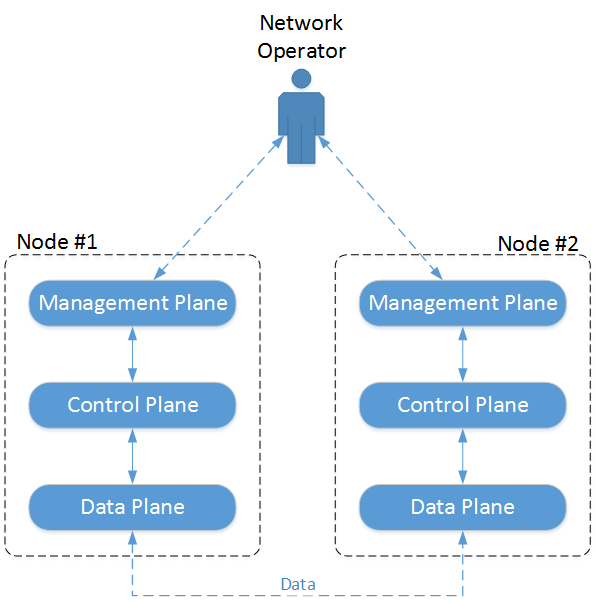
\includegraphics[scale=0.65]{Traditional_Network_Architecture}
	\caption{Two node network according to the traditional network node architecture.}
	\label{fig:Traditional_Network_Architecture}
\end{figure}
%
Having these three planes tightly-coupled and implemented in the network nodes is the reason behind both the box-centric configuration style and vendor-specific configuration workflow and interface.
\gls{SDN} decouples these planes from one another, defining the abstraction of \emph{Specification}, corresponding to the management plane functionality, \emph{Distribution}, corresponding to the control plane functionality, and \emph{Forwarding}, corresponding to the data plane functionality.
By doing so, this new architectural concept makes it possible to logically centralize the \emph{Specification} and \emph{Distribution} while keeping the \emph{Forwarding} implemented in the network nodes\cite{Kreutz2014}\cite{OFWP},\cite{OpenNetworkingFoundation} thus creating the premises for a network infrastructure that harnesses the benefits of both distributed data forwarding and centralized management, dismissing today's decentralized network management style.\\
%
The second core feature of \gls{SDN} is the ability to programmatically configure the network, which is accomplished by having the Specification expose a set of \glspl{API} to be consumed by network applications.
These \glspl{API} are generally capable of exposing the network topology through global and abstracted views, as well as providing methods of global policy definition and common network functionality such as routing, access control and bandwidth management\cite{OFWP}.
The policies are then applied to the appropriate network nodes by the \emph{Distribution} through the use of a communication protocol implemented both on this abstraction and on the network elements.\\
%
These two core concepts lead to the definition of the architecture of \gls{SDN} in three layers, the \emph{Application} layer, the \emph{Control} layer and the \emph{Infrastructure} layer \cite{OpenNetworkingFoundation}\cite{Kreutz2014} as depicted in Figure \ref{fig:SDN_Architecture}.
\begin{figure}
	\centering
	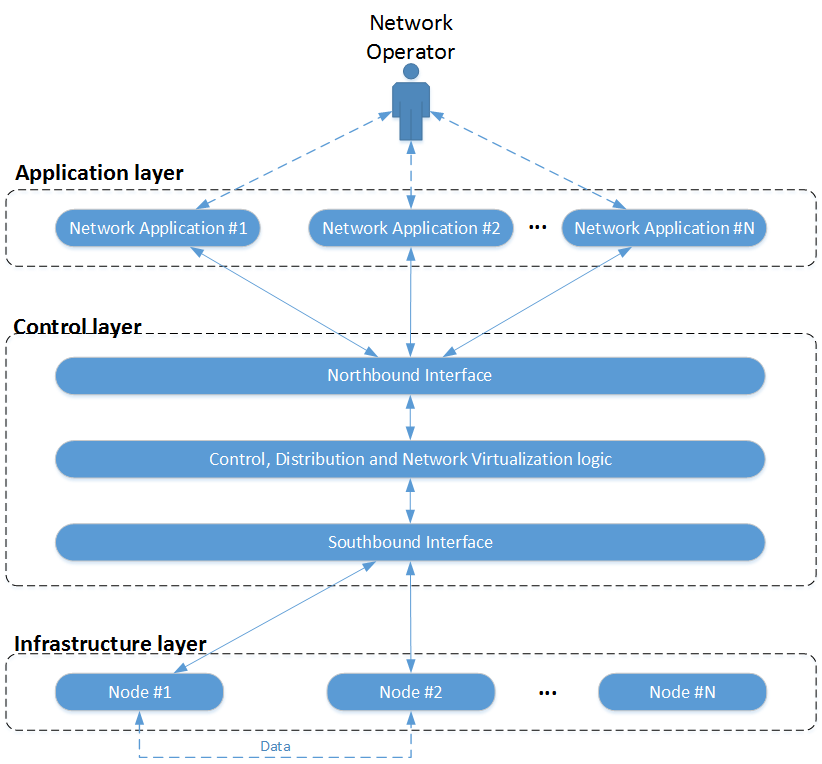
\includegraphics[scale=0.70]{SDN_Architecture}
	\caption{Two node network according to the SDN architecture.}
	\label{fig:SDN_Architecture}
\end{figure}
The Infrastructure layer is where all the network nodes reside, performing all the Forwarding functions.
The Control layer encompasses the Specification and the Distribution, therefore dealing with all the network management and control mechanisms.
The Application layer is where the network applications reside.
These applications define the network policies through the Control's northbound \glspl{API}, taking into account factors such as (but not restricted to) network topology and the network operator input.\\
This three-layered architecture, depicted in figure \ref{fig:SDN_Architecture}, is commonly extended to a for-layered architecture by breaking the Control layer in two, creating a layer solely for network virtualization that sits between the Control and Infrastructure layers.\\
%
The implementation of the Control layer is known as \gls{SDN} controller or \gls{NOS}, and it is the main building block for Software-Defined Networks.
A \gls{SDN} Controller exposes a northbound interface, intended for interaction with network applications corresponding to the Specification functionality, a southbound interface intended for interaction with the network elements in the scope of the Distribution functionality, and in some cases eastbound/westbound interfaces for integration with other \gls{SDN} controllers (mostly seen in distributed controllers)\cite{Kreutz2014}.
The southbound interface must implement the same protocol as network elements do in order for network programmability to work, effectively making the definition of good standard protocols and acceptance of said protocol by vendors a key point of action for \gls{SDN} to prosper.\\
%
By comparing figures \ref{fig:Traditional_Network_Architecture} and \ref{fig:SDN_Architecture} it is easy to understand that this new architecture simplifies management by having it done in a single point (Control layer) instead of multiple points (network nodes) and fosters innovation as the implementation of new network policies or custom network behavior can now be promptly implemented by introducing an application to do so without the need of knowing how it will be implemented in the network infrastructure or even of how the network infrastructure is composed.
Furthermore, applications can be written to dynamically adjust network policies according to the network status without the need for Human intervention, thus drastically reducing the time required to adjust network policies upon network events such as topology changes and therefore potentially increasing the effectiveness of said policies should the event pose a security threat or risk of service outage.
Another inherent advantage of this solution is the consistency of the policy throughout the network, seeing that the policy is now defined by the network operator through a network application in a global scope and in a single point, therefore eliminating inconsistencies in configurations between different network nodes.\\
%

There are currently several implementations for SD\gls{SDN}N controllers such as OpenDaylight\cite{OpenDaylight}, Floodlight\cite{Floodlight} and ONOS\cite{ControllerComparison} \cite{Kreutz2014}, as well as southbound interfaces such as OpenFlow, POF, ForCES and OpFlex \cite{Kreutz2014}.
Although at first it might not be obvious at first, the fact that multiple southbound interfaces exist presents itself as an issue, given that either network elements or \gls{SDN} controllers must implement more than one of them in order to achieve compatibility between \gls{SDN} controllers and network elements.
Because there is now a dominant southbound interface - OpenFlow - the vast majority of network elements implementing the \gls{SDN} architecture are implementing only OpenFlow.\\
%
The \gls{ONF} has made OpenFlow a standard protocol and is working on standardizing the northbound interfaces\cite{OFWP}, which will make network applications controller-agnostic, which in turn will streamline development and make application portability possible.\\
%
Today's data center's multitenancy is growing as a consequence of \gls{IaaS} and as such infrastructure virtualization becomes increasingly important both for security and service reasons.
With more and more companies migrating their \gls{IT} infrastructure to private cloud infrastructures, network virtualization starts to gain new perspectives as traffic isolation is not enough, with support for custom tenant network topologies being required to smooth the transition.
There are also several network virtualization implementations for \gls{SDN} such as FlowVisor\cite{Sherwooda}\cite{Sherwood} and OpenVirteX\cite{Kreutz2014}.
These implementations are analogous to the hypervisors in \gls{IT} virtualization, sitting between the \gls{SDN} controller and the network elements, acting as a proxy for the communications between both.
Multiple \gls{SDN} controllers are allowed to interact with the same instance of the virtualization layer, one for each virtual network.\\
%
\subsection{Southbound interfaces}
\label{subsection:sdn-southbound-interfaces}
The \gls{SDN} architecture is possible due to the existence of protocols for programming the forwarding plane, also referred to as southbound interfaces (from a \gls{SDN} controller perspective).
There are currently several protocols, such as \gls{POF}\cite{POF}, \gls{ForCES}\cite{ForCES}, OpFlex\cite{OpFlex} and OpenFlow\cite{OFWP}.
%
\gls{POF} attempts to enhance the forwarding plane programmability by defining generic matching rules that make use of offset definitions instead of packet header definitions.
In practice, matching in \gls{POF} is performed against a sequence of bits with specified length in a packet starting at a given position, effectively allowing the definition of matches against any packet header regardless of the protocol\cite{POF}.
%
\gls{ForCES}, despite also aiming at decoupling control from forwarding, does not require the existence of a network controller and instead the control is allowed to remain in the network nodes\cite{Kreutz2014}.
%
OpFlex mixes concepts from both OpenFlow and \gls{ForCES}, having the management being centralized while the control remains distributed in the network elements \cite{Duffy2014}.\\
%

OpenFlow, the most prominent of them, is a standard protocol for forwarding plane programming, defined by the \gls{ONF} and designed for Ethernet networks\cite{OFWP}.
It is analogous to the Instruction Set of a \gls{CPU} in the sense that it defines primitives that can be used by external applications to program the network node much like it is done with \glspl{CPU}\cite{OFWP}.
Forwarding decisions are based in the notion of flows, which according to the \gls{IETF} is "a sequence of packets from a sending application to a receiving application"\cite{IETFFLOW}.
OpenFlow is supported by several vendors such as Cisco\cite{CISCOOF}, Juniper\cite{JUNOSOF}, HP\cite{HPVAN} and Alcatel-Lucent\cite{ALUOF}.\\
%
%*** OVSDB vs OF-CONFIG
While the OpenFlow protocol allows for forwarding plane programming, some network management aspects are not entirely bound to forwarding decisions.
Some of these aspects include turning network ports on and off and establishing tunnels between network elements.
There are however other southbound protocols that introduce these management capabilities and rely on OpenFlow to implement forwarding plane programming, namely the \gls{OVSDB} and the \gls{OF-CONFIG}\cite{OVSDBvsOFCONFIG}.
\gls{OVSDB} is a component of Open vSwitch and it is designed to manage Open vSwitch implementations.
\gls{OF-CONFIG} is defined by the \gls{ONF} specifically to be used alongside with OpenFlow and may be implemented in both software or hardware network element implementations.
%
%
% OF
\section{OpenFlow}
\label{section:openflow}
Having had several versions released since 2008 when version 0.8.0 debuted, OpenFlow is currently on version 1.5\cite{OF15}.
However, because changes made from version 1.3 to version 1.5\cite{OF15}\cite{OF13} are not relevant to the scope of this work and because both hardware and software switch implementations mainly implement version 1.3 we will focus on version 1.3 for the purpose of this work.\\
%
As previously mentioned, there are now several available implementations of OpenFlow-enabled network elements, however OpenFlow implementation and traditional forwarding planes implementations are not mutually exclusive, thus the definitions of \emph{OpenFlow-only} network elements (which implement only the OpenFlow forwarding plane) and \emph{OpenFlow-hybrid} network elements (which implement both the OpenFlow and legacy forwarding planes).
In the later, OpenFlow specifies means of forwarding traffic from the OpenFlow forwarding plane and into the legacy forwarding plane\cite{OF13}.
This is in fact a major upside to OpenFlow adoption, as it makes the adoption of OpenFlow by hardware vendors as easy as releasing a new software version that implements the OpenFlow forwarding plane on top of existing network hardware, and allows adopters to gradually roll-out OpenFlow in existing networks possibly with existing network hardware.\\
%
The OpenFlow specification defines the architecture of an OpenFlow switch implementation in three main building blocks: the \emph{OpenFlow Channel}, the \emph{Processing Pipeline} and the \emph{Group Table} as depicted in figure \ref{fig:OF_switch_arch}.
\begin{figure}
	\centering
	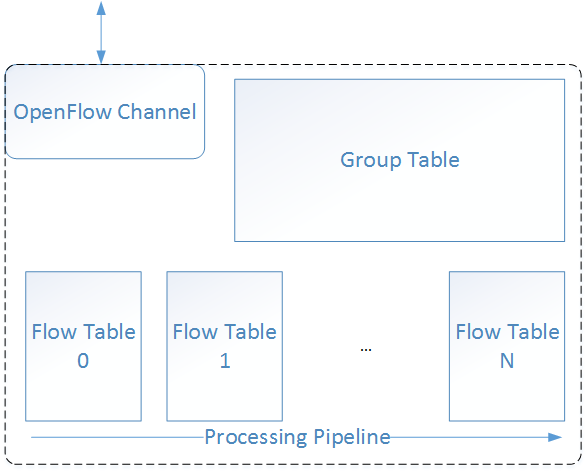
\includegraphics[scale=0.65]{OF_switch_arch}
	\caption{OpenFlow switch architecture.}
	\label{fig:OF_switch_arch}
\end{figure}
The \emph{OpenFlow Channel} defines the interface for communications between the OpenFlow switch and the \gls{SDN} controller, through which controllers can statically or dynamically create, modify and remove \emph{flow entries} from \emph{flow tables}.
Further detail on the differences between static and dynamic flow entry programming will be addressed later in this document.
All communications between an OpenFlow switch and an \gls{SDN} controller are encrypted by default using \gls{TLS} even though it is possible use plain \gls{TCP}\cite{OF13}.
These communications are always initiated by the OpenFlow switch, and each switch may have one or more \gls{SDN} controller \gls{IPAddress} specified in its base configuration.
The OpenFlow switch is required to maintain active connections witch all configured \gls{SDN} controllers simultaneously. Because multiple \gls{SDN} controllers may be configured in a single switch, each controller is assigned one of three possible roles: \emph{Master}, \emph{Slave} or \emph{Equal} \cite{OF13}.\\
The Master role grants the \gls{SDN} controller full management access to the switch, allowing it to program flow entries and receive notifications of events occurring on the switch, such as flow entries expiring and port status updates.
There can be at most one \gls{SDN} controller configured as master per switch.
The Slave role grants the \gls{SDN} controller with read-only access to the switch, allowing it to receive only port status updates.
Any \gls{SDN} controller instance that is already connected to the switch can request to change role from slave to master, at which point the instance that previously held the master role will be updated to the slave role.
This mechanism provides a fault tolerance mechanism by allowing for the existence of Active-Standby \gls{SDN} controller clusters. 
The Equal role is essentially the same as the Master role, with the exception of allowing one switch to be connected to multiple \gls{SDN} controllers in Equal role.
This specific role aims at introducing a mechanism for fault tolerance but also load balancing, requiring however that the \gls{SDN} controllers coordinate with each-other.\\
The \emph{Processing Pipeline} is composed of several \emph{flow tables} (with a required minimum of one), each containing a set of \emph{flow entries}.
A \emph{Flow entry} is defined by a set of fields, namely:
\begin{itemize}
	\item \textbf{Priority}, which defines its precedence over other flow entries in the same table, with the highest value taking precedence
	\item \textbf{Match fields} consisting of header patterns that when positively matched against a packet identify a flow
	\item A set of \textbf{instructions} that determine the course of action the switch should take to handle the flow
	\item \textbf{Timeouts} defining for how long the flow entry is to be maintained in the flow table, namely a \emph{hard timeout} which forces the flow entry to be removed $\Delta$ seconds after it was installed and a \emph{soft timeout} specifies for how long the flow entry shall be kept after the last matching packet as been matched
	\item \textbf{Counters} that increment each time a packet is successfully matched against the flow entry
	\item \textbf{Cookies}, which are used exclusively by the \gls{SDN} controller to annotate the flow entry
\end{itemize}
%
For each flow table there might be one special flow entry that matches all packets and with a priority of zero, called the \emph{table-miss flow entry} and it defines the default action set to be taken by the switch for any given packet.
Flow matching is performed in a one way direction, starting in flow table \emph{0} (which is the only mandatory flow table) and ending with either a set of actions to be executed (defined by matching entries) or alternatively dropping the packet.
This means that once processing has reached table \emph{n}, it can then either resume processing in table \emph{m} where \emph{m $>$ n} if the matching flow entry defined such instruction, or execute the actions in the instruction set defined by matching entries in tables \emph{0} through \emph{n}.
If no entries that match the packet occurred then either there is a table-miss flow, usually redirecting the packet to the \gls{SDN} controller or simply resuming the pipeline processing in the next table, or the switch drops the packet completely.
%
Last but not least, the \emph{Group Table} contains \emph{group entries}.
\emph{Group entries} allow the definition of \emph{action buckets}, which are defined by a \emph{Group Identifier} uniquely identifying the group entry, a \emph{Group Type} defining the behavior of the Group entry, and a set of \emph{Action Buckets} which are themselves sets of actions to be executed by the switch.
\emph{Group entries} are somewhat analogous to action macros, simplifying forwarding functions such as broadcast and multicast\cite{OF13}.\\
%
An OpenFlow switch may also implement a \emph{meter table} allowing for the implementation of simple \gls{QoS} features such as queue management and rate limiting\cite{OF13}.\\
The aforementioned mechanisms grant OpenFlow the ability to perform highly granular control over how specific flows should traverse the network, enabling the differentiation of traffic according to its profile\cite{OFWP}.
Consequently, network protocol implementations on network elements become increasingly deprecated, leading to the dismissal of said implementations in favor of OpenFlow forwarding plane implementations instead, thus having for the forwarding decisions being programmed from the \gls{SDN} controller according to the global policies set for the network\cite{OFWP}.\\
%
% OF Flow programming
\subsection{OpenFlow flow programming}
\label{subsection:openflow-flow-programming}
% Static vs Dynamic flows
%
\begin{figure}
	\centering
	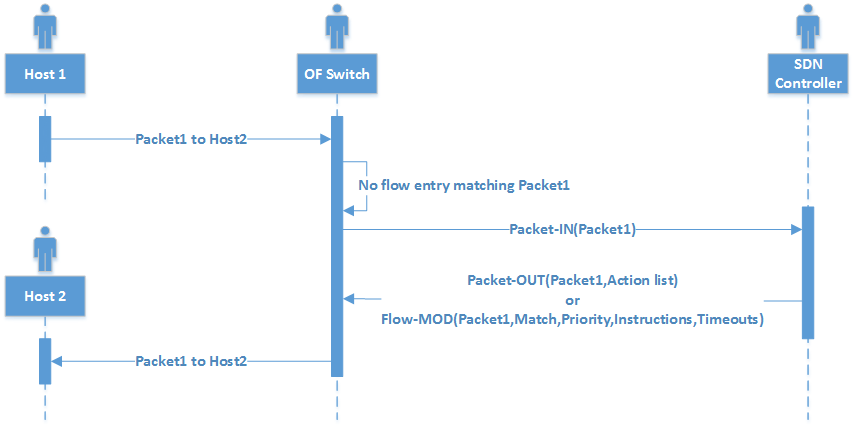
\includegraphics[scale=0.65]{OF_dynamic_flow_programming}
	\caption{OpenFlow reactive flow programming}
	\label{fig:OF_dynamic_flow_programming}
\end{figure}
%
\gls{SDN} controllers may program flow entries in OpenFlow switches by issuing \emph{flow table modification} messages.
These messages allow the \gls{SDN} controller to manipulate flow tables by adding new flow entries and modifying or removing existing flow entries.
Flow entry additions performed by the \gls{SDN} controller by issuing a flow table modification message to predefine the forwarding behavior ahead of data transmission is referred to as static flow entries and configures the proactive flow programming paradigm.
These flow entries usually have both their hard and soft timeouts set to zero, meaning that they will not expire\cite{OF13}.
Having these flow entries present in the flow tables enable the traffic to be forwarded immediately when reaching the OpenFlow switch.
However, it has the disadvantages of having to preprogram flow entries to cover every single flow possible according to the global network policy, which leads to a quick exhaustion of the flow tables available in the switch.
Furthermore, the action set being preprogrammed might not be optimal for a particular flow being processed at a particular point in time.
A typical usage of static flow entries are the table-miss flow entries, which have already been discussed.
%
Table-miss flow entries, defining an instruction to forward the packet to the \gls{SDN} controller through a \emph{packet-in} message, on the other hand enable the \gls{SDN} controller to examine the packet and define the proper actions to be executed by the switch in a reactive fashion.
The \gls{SDN} controller may respond to this message with either a \emph{packet-out} message defining the actions to be executed exclusively for that packet or alternatively with a flow table modification message that will create a new flow entry to handle all the packets matching that flow, including the original packet included in the packet-in message\cite{OF13}, as depicted in figure \ref{fig:OF_dynamic_flow_programming}.
%
The resulting flow entries are referred to as \emph{dynamic flow entries}, and it is one of the most powerful features of OpenFlow as it allows for forwarding decision-making to be performed by a centralized system that has global view and control over the network - the SDN Controller - thus configuring the reactive flow programming paradigm.
This however comes with a considerable computational cost, since every first packet of each new flow being admitted into the network must be sent to and evaluated by the \gls{SDN} controller which in turn will instruct the switch(es) on how to behave for that flow.
When considering large-scale networks, such as that of a big data center, the amount of packets that must be sent to and processed by the controller is far too great to be handled by a single controller instance, therefore rendering this approach unfeasible.
%
%TEX root = ../dissertation.tex

\chapter{Architecture}
\label{chapter:architecture}
\section{OpenFlow SDN controller cluster}
\label{section:SDN-controller-cluster}
As previously mentioned, the OpenFlow specification provides mechanisms for resilience and load balancing across multiple \gls{SDN} controller instances.
OpenFlow allows for an OpenFlow switch to be connected to several \gls{SDN} controllers simultaneously, however, the latter are expected to have some sort of coordination between them in order to achieve load balancing, which is achieved by exposing eastbound/westbound \glspl{API} to be consumed by neighboring controllers within the same management domain.
This approach also requires that every OpenFlow switch within the management domain be reconfigure every time an instance is added or removed from the \gls{SDN} controller cluster.\\
%
Having the instances coordinated with each other and keep consistent states in a distributed environment requires therefore a controller cluster and configures an architecture such that of figure \ref{fig:sdn_simple_clustering}.\\
%
\begin{figure}
	\centering
	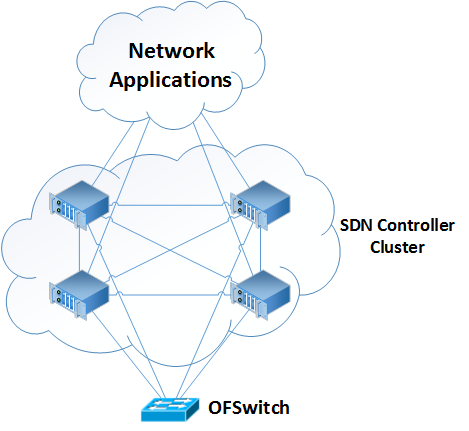
\includegraphics[scale=0.65]{sdn_simple_clustering}
	\caption{OpenFlow SDN controller clustering}
	\label{fig:sdn_simple_clustering}
\end{figure}
%
The resulting cluster should support key aspects of the \gls{SDN} controller component, such as keep a global view and management scope.
Because the goal is to perform load balancing between all instances, each instance will be actively managing any given number of OpenFlow switches in the same management domain, and therefore the network state is distributed in nature.
In order to maintain the aforementioned key aspect of \gls{SDN} controllers, active instances must propagate their \gls{MIB} on to their cluster peers and be prepared to update their own \gls{MIB} with updates issued by their peers.
The propagation of these updates must be triggered at least when network events are detected and when new adjacencies between OpenFlow switches controlled by different instances are detected.
When a instance propagates updates to other peer instances, it must guarantee causal consistency.\\
%

%!TEX root = ../dissertation.tex

\chapter{Implementation}
\label{chapter:implementation}
To demonstrate the architecture feasibility and validity, a proof of concept implementation has been developed by means of extending an existing \gls{SDN} controller and integrating a Linux kernel module for clustering.\\
%
The requirements set for the choice of the controller were controller completeness, popularity and availability of source code, which lead to a final decision between OpenDaylight\cite{OpenDaylight} and Floodlight\cite{Floodlight}\cite{Kreutz2014}\cite{ControllerComparison}.
%Justify choice of Floodlight
While both OpenDaylight and Floodlight are modular open-source \gls{SDN} controllers implemented in Java, highly popular and supported by major players in the networking industry\cite{OpenDaylight}\cite{Floodlight}, however, at the time of the decision, Floodlight, which was at version 1.1, had a more stable implementation when compared with the OpenDaylight, which was at release Helium.
OpenDaylight also offers support for multiple Southbound Interface protocols, which while falling outside the scope of this work renders the platforms architecture more complex than that of Floodlight, and would therefore add more complexity to the implementation.
For these reasons, Floodlight was chosen as a basis for the implementation of proof of concept for the proposed architecture.\\
%
\section{Elastic SDN controller cluster}
\label{section:SDN-controller-cluster-implementation}
% Floodlight
Floodlight is a modular implementation of a \gls{SDN} controller developed by Big Switch Networks using the Java language, and is currently in version 1.1.
Floodlight shares its core implementation with Big Switch Networks's own Big Network Controller\cite{Floodlight}.
It offers stable support for OpenFlow versions 1.0 and 1.3 and experimental support for versions 1.1, 1.2 and 1.4 through OpenFlowJ Loxi, a library that encapsulates the OpenFlow protocol and exposes functionality through a protocol version agnostic \gls{API}\cite{LoxiGen}.\\
Floodlight's architecture is highly modular, composed by a base \emph{Module Loading System} that loads a set of registered modules, allowing for the establishment of inter-module dependencies as well as service exposure and consumption by registered modules\cite{FLArch}.
There are a set of \emph{Controller Modules} which implement core \gls{SDN} controller functionality which is then either exposed by service \glspl{API} or by propagating as events to registered listener modules, thus enabling an event-driven programming model.
These modules implement features such as OpenFlow switch management connection handling (FloodlightProvider and OFSwitchManager modules), inter-switch link discovery through \gls{LLDP} and \gls{BDDP} (LinkDiscoveryManager module), network host discovery and tracking through packet-in inspection (DeviceManagerImpl module) and network topology and routing service (TopologyService module).\\
Floodlight defines a unique device as a (\gls{VLAN};\gls{MACAddress}) pair and considers that there may be at most one attachment point per network domain \cite{FLArch}.
In order to maintain compatibility the same concepts were taken into consideration for the implementation of the proof of concept.\\
%NOTE: DeviceManagerImpl "By default the entity classifier uses MAC address and VLAN to identify a device. These two properties will define what is unique as a device. (...) A device can have as many as one attachment point per OpenFlow island, where an island is defined as a strongly connected set of OpenFlow switches talking to the same Floodlight controller."
%
\subsection{Proof of concept implementation}
\label{subsection:poc-module}
%
% Highlevel description
The proof of concept implementation followed Floodlight's architectural design.
A floodlight module was therefor implemented, encapsulating all the clustering concepts stated in chapter \ref*{chapter:architecture} section \ref{section:SDN-controller-cluster} and both providing \glspl{API} and triggering events to registered listeners.
The main building blocks composing the developed module depicted in figure \ref{fig:amorphous_block_diagram} are as follows:
%
\begin{figure}
	\centering
	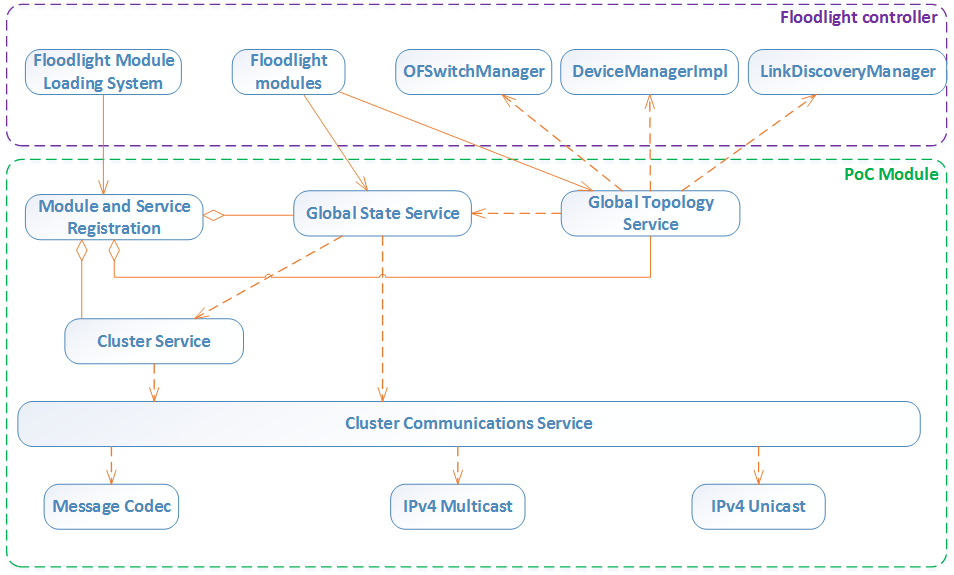
\includegraphics[scale=0.65]{amorphous_block_diagram}
	\caption{Proof of concept implementation high level block diagram}
	\label{fig:amorphous_block_diagram}
\end{figure}
%
\begin{itemize}
	\item \textbf{Module and Service registration:} Handles all the tasks necessary to integrate with the Floodlight controller, including component initialization, declaring dependencies and exposing the services provided by both Global State Service and Global Topology Service by implementing the IFloodlightModule interface, which is then used by the Floodlight Module Loading System to register and execute the module.
	%
	\item \textbf{Global State Service:} Handles the global state of the \gls{MIB} and exposes an \gls{API} to provide message exchange between Floodlight modules executed in different instances of the cluster, therefore allowing for the extension and enhancement of the distributed environment properties to module specific implementations. The message exchange \gls{API} provided is based on the concept of named message queues, in which a module registers in a queue and is allowed to send messages to and listen for incoming messages on the queue. This module depends on the Cluster Communications Service to exchange messages with peer controller instances and on the Cluster Service in order to determine the address of the destination peer and whether or not a peer is a member of the cluster.
	%
	\item \textbf{Global Topology Service:} Locally, it provides the same services as the TopologyService module by exposing an \gls{API} to be consumed by other Floodlight modules and triggering events upon topology changes, using however the Global State Service's \gls{MIB} instead of the local \gls{MIB}. It also listens for local topology changes, such as new OpenFlow switch connections, new inter-switch links and hosts, updating its \gls{MIB} and propagating the changes to peer instances accordingly. This block registers to a special queue in Global State Service reserved for the exchange of the messages specified in table \ref{table:cluster-message-spec} under the scope of gls{MIB} update. All messages queued for sending through the exposed \gls{API} are sent encapsulated (and de-encapsulated when received before being registered to the corresponding queue) within a special purpose container message that holds properties such as the queue identifier.
	%
	\item \textbf{Cluster Service:} This block is responsible for all the clustering logic such as that of the registration of peer cluster instances (including the registration of the local instance with existing ones) described in chapter \ref*{chapter:architecture} section \ref{section:SDN-controller-cluster} and the exchanging and processing of all the messages stated in table \ref{table:cluster-message-spec} under the scope of cluster membership. Messages are sent and received using the \gls{API} provided by the Cluster Communications Service.
	%
	\item \textbf{Cluster Communications Service:} Encapsulates all of the network communication details, providing a unified \gls{API} to both Cluster Service and Global State Service, thus enabling them to send and receive messages to and from peer controller instances. The messages are encoded/decoded to a suiting transmission format by the Message Codec block, and then sent and received by the network access specific implementations. The network access is done using \gls{IPv4} seeing that it is the most widespread network protocol. The network access specific implementations are contained in the IPv4 Multicast and IPv4 Unicast blocks, allowing for the easy replacement of the network protocol used simply by implementing new blocks that expose the same \gls{API}.
	%
	\item \textbf{Message Codec:} Encodes and decodes messages to a suitable format to be sent through the network, which is essentially an array of bytes. In this implementation, the method chosen to encode/decode is the serialization of Java objects, however, any other method can be implemented such as \gls{JSON} or otherwise a special purpose Application Layer\footnote{Considering the \gls{OSI} model} protocol in order to make messages compatible with any \gls{SDN} controller implementation, regardless of the programming language it was developed in.
	%
	\item \textbf{IPv4 Multicast:} All of the \gls{IPv4} multicast implementation is contained within this block. The multicast group used for this implementation is 224.0.1.20, which is a special group address reserved for private experiments\cite{ReservedMulticastGroups} within the multicast addresses block for portocol traffic that is allowed to be forwarded through the internet\cite{rfc5771}.
	%
	\item \textbf{IPv4 Unicast:} This block implements all of the \gls{IPv4} unicast using only \gls{TCP} as it provides guaranteed delivery independently of message size.
\end{itemize}
%
% Optimizations
The group communication paradigm specified in chapter \ref*{chapter:architecture} section \ref{section:SDN-controller-cluster} is implemented using the \gls{IPv4} multicast mechanism provided by the IPv4 Multicast block, which presented an additional challenge as \gls{IPv4} multicast does not provide a connection oriented communication, therefore requiring for manual fragmentation, ordering and reassembly of messages with size greater than the \gls{MTU}.
In order to overcome this limitation without going into complex message delivery implementations while still keeping the desired properties of group communication, a workaround was implemented in the Cluster Communications Service block in which if the size of a message destined to all cluster members is large enough not to fit into a single packet (in which case the IPv4 Multicast block will raise an exception), instead of using the multicast mechanism, unicast \gls{TCP} sessions are established to all registered clustered members, conveying the message through these sessions.
All of the messages specified in table \ref{table:cluster-message-spec} within the scope of cluster membership and targeted at the whole cluster are guaranteed to fit in a message which size is lesser than the \gls{MTU} and are therefore not affected by this workaround, thus keeping the group communication properties required for cluster formation and maintenance intact.\\
In order to reduce the amount of data transmitted and at the same time provide a fail recovery mechanism, the Join cluster and Instance health messages defined in table \ref{table:cluster-message-spec} were merged into the a single message (Join cluster), having each instance the responsibility differentiating the message purpose according to whether the instance sending the message was already registered (in which case a timestamp indicating the last time the instance reported activity is updated) or not (in which case the registration process is executed).\\
%
In order for inter-switch links connecting OpenFlow switches controller by different instances to be properly detected and registered into the global topology, the LinkDiscoveryManager module had to altered in such a way that the incoming \gls{LLDP} packets sent by other controller instances are processes according to the topology made available by the Global topology Service instead.
This represents the only change required to the Floodlight core modules in order for the proof of concept implementation to work.
%
\subsection{Distributed network policy module}
\label{subsection:poc-application}
%
Floodlight comes bundled with a set of network applications that provide network policy functionality out the box.
One of these applications is the Forwarding module, which is a module providing a default policy of permit any to any communications, installing flow entries to allow flows in a reactive fashion\cite{FLFwd}.\\
The nature of this modules makes it a perfect test subject for the proposed architecture, however, in order to better demonstrate the full potential of the proposed architecture this module was extended to take advantage of the inter-instance communication mechanism provided by the Global State Service so that the forwarding policy is only computed on the \gls{SDN} controller instance managing the OpenFlow switch to which the device that initiates the flow is connected to. Controller instances managing other OpenFlow switches in the path the flow takes to traverse the network are simply instructed which flow entries to add to which switches instead of having to compute the policy by themselves.
This approach increases scalability as the computational cost of determining the actions to be performed for any given flow is only inflicted in one controller instance, leaving other controller instances free to compute the flows being admitted into the network through OpenFlow switches that they control directly.\\
This extended version of the Forwarding module, registers to a queue named after itself using the Global State Service \gls{API} which will be used to exchange messages coordinating policy programming actions throughout the network.
Upon receiving a Packet-In for a packet that hit the table miss flow, it consumes the \gls{API} of the Global Topology Service in order to determine if the destination device is already known in the topology (at global scope) and if so which is the shortest path between the source and destination devices.
Should the destination device be unknown to the topology, the packet is flooded to all ports of the corresponding broadcast domain in the local OpenFlow switch and the process terminates.
If however the destination is known in the global topology, it takes the path computed by the Global Topology Service and in turn computes the flow entry to be programmed in each OpenFlow switch pertaining to path and sends out Flow Programming Request messages to the controller instances managing the involved OpenFlow switches that are not locally managed.
Flow Programming Requests are then processed by the receiving instances which notify the instance that sent it with a Flow Programming Confirmation message upon completion.
The instance that computed the policy is only allowed to program the flow entry in the OpenFlow switch that triggered the Packet-In after receiving Flow Programming Confirmation messages from all remote instances involved, thus making sure that there will be no other Packet-In triggered in the path.
%
%TODO: Lamport clocks to guarantee causal consistency and avoid loss of information during the sync process (message buffer)
%
\section{Request Router}
\label{section:request-router}
The request router component was implemented by integrating Linux virtual machines running Linux kernel 3.16 compiled with the \gls{IPVS} module, with the Elastic \gls{SDN} controller cluster.
The \gls{IPVS} module, pertaining to the Linux Virtual Server Project, provides an efficient kernel-mode \gls{OSI} layer 4 switching facility, suited to load balance client connections between several clustered servers \cite{LVS}.
In order to implement the \gls{anycast} communication paradigm, it is assumed that the core network infrastructure to which the OpenFlow management interfaces and \gls{SDN} controller instances are connected to support the \gls{BGP} routing protocol and are able to peer with request router instances.
The configuration of the network is not within the scope of this work.
%
\subsection{Linux Virtual Server}
%TODO: Linux LVS
The Linux Virtual Server project, in particular the \gls{IPVS} module, provides an out of the box load balance facility for client-server applications connecting through the network and using the \gls{IPv4} stack.
This module, implemented as a kernel module, introduces minimal overhead in the client-server communication and can be deployed as a cluster, in which mode forwarding states will be synchronized between cluster members, thus allowing for the required infrastructure resiliency seeing that a request router instance failure will not impact normal operation as its peer instance is able to take over the forwarding function seamlessly \cite{LVSSync}.\\
%
%TODO: IPVS modes http://www.linuxvirtualserver.org/how.html : Because of DST -> VS/DR
The load balancing is performed at the Transport Layer of the \gls{OSI} model, supporting both \gls{UDP} and \gls{TCP} protocols.
IPVS receives the connection data from the client for a configured service cluster and forwards it to the one of the servers available for that cluster in one of three possible ways\cite{IPVSHow}:
\begin{itemize}
	\item In \textbf{\gls{NAT} mode}, \gls{IPVS} terminates the client connection and initiates a new connection with the service cluster instance determined by the load balance algorithm, forwarding all the packets received from the client to the server, masquerading however the source \gls{IPAddress}, effectively forcing data communications to go through the load balancer in both ways. While this mode offers the advantage of allowing the service cluster servers to be located anywhere on the network and requiring no configuration on the clients nor the servers, it has limited scaling capabilities as \gls{NAT} itself is limited when it comes to scaling
	%
	\item In \textbf{IP Tunneling mode}, \gls{IPVS} does not terminate the client-server communication and instead encapsulates the data being received from the client inside an IP-IP packet and forwards it to the service cluster instance determined by the load balance algorithm. This mode also offers the advantage of allowing the service cluster servers to be located anywhere on the network, requiring however that the servers support the IP-IP tunneling (which introduces minimal overhead) and the configuration of loopback interfaces with the service cluster \gls{IPAddress} in all of the service cluster servers. It is however much more scalable than \gls{NAT} mode, since this mode does not perform \gls{NAT} nor does it process packets coming from the server to the client.
	%
	\item In \textbf{Direct Routing mode}, \gls{IPVS} behaves essentially in the same way as in the IP Tunneling mode, however instead of performing encapsulation the load balancer is instead required to be on the same \gls{OSI} layer 2 as the service cluster servers, forwarding the packets received by the client directly to the service cluster instance determined by the load balance algorithm. While this mode offers the same advantages as the IP Tunneling mode and without the IP Tunneling drawback, the requirement of being in the same \gls{OSI} layer 2 as the service cluster server represents a limitation in terms of solution design.
	%
\end{itemize}	
%
Both the IP Tunneling and Direct Routing modes met the requirements set for the request router component, however, the IP Tunneling mode chosen for this implementation since it does not limit the deployment topology and IP-IP tunneling is natively supported in modern Linux kernels.
It is worth to note however that the forwarding mode is determined by server and not by service cluster, which means that it is possible to use more than one of these modes simultaneously for different servers in the same service cluster.\\
%
IPVS also offers a number of load balance algorithms that can be used to determine to which service cluster instance the client connection should be forwarded to:
%
\begin{itemize}
	\item The \textbf{Round Robin} algorithm iterates through the configured servers, assigning client connections equally to each.
	%
	\item The \textbf{Weighted Round Robin} algorithm allows the definition of weights per server, which are then taken into account when assigning client connections such that servers with higher weight are assigned more connections.
	%
	\item The \textbf{Least-Connections} algorithm assigns new client connections to the server with least active connections.
	%
	\item The \textbf{Weighted Least-Connections} algorithm is the default algorithm and like the Weighted Round Robin it allows for the definition of weights per server. It then assigns new client connections to the server with the lowest Connections to Weight ratio.
	%
	\item The \textbf{Locality-Based Least-Connections} algorithm assigns incoming connections to the same server if it is not overloaded or unavailable, in which case it assigns the connection to another server with fewer connections.
	%
	\item The \textbf{Locality-Based Least-Connection with Replication} algorithm defines a server set that can serve the client's request and forwards the packets to the server in that set with least active connections. If all servers in the set are overloaded, a new server belonging to the service cluster is added to the set of servers that can serve the client and the packets are forwarded to that server.
	%
	\item The \textbf{Destination Hashing} algorithm consistently assigns server by looking up a hash table using the service cluster \gls{IPAddress} as key.
	%
	\item The \textbf{Source Hashing} algorithm consistently assigns server by looking up a hash table using the client's \gls{IPAddress} as key.
	%
	\item The \textbf{Shortest Expected Delay} algorithm assigns client connections to the server that is expected to have the shortest delay, which is estimated by $\frac{(C + 1)}{U}$ where C is the number of connections for the server and U the Weight assigned to the server.
	%
	\item The \textbf{Never Queue} algorithm assigns client connections to on of the idling servers. Should there be no idling server the Shortest Expected Delay is used to assign a server.
	%
\end{itemize}
%
The optimal algorithm according to the requirements set for the request router would be the Source Hashing since it guarantees a deterministic load balancing decision, however, for the purposes of testing this implementation using a network emulator Least Connections was chosen instead seeing that the Source Hashing would always assign the same server since the source \gls{IPAddress} would always be the same for all OpenFlow switches (that of the emulator).
%
\subsection{Elastic Cluster Integration}
%TODO: Request Router component (Multicast integration)
The request router must integrate with the \gls{SDN} controller elastic cluster in order to determine the set of active controller instances to which it can forward OpenFlow switch connections.
To do that, a new component was developed, much like the developed Floodlight module, joining also the same multicast group in order to receive Join messages through which it infers the active set of controller instances.
Because the message encondig/decoding is performed using Java's object serialization, this components implementation necessarily had to be made using the Java language as well.
The building blocks of the component are depicted in figure \ref{fig:rr_block_diagram} and are as follows:
%
\begin{figure}
	\centering
	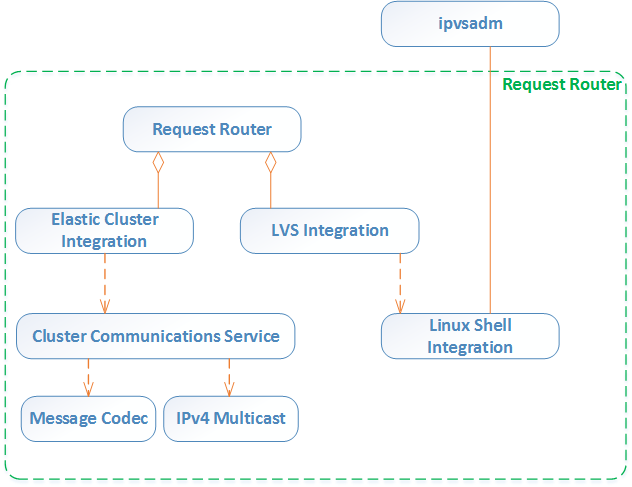
\includegraphics[scale=0.65]{rr_block_diagram}
	\caption{Request Router integration component high level block diagram}
	\label{fig:rr_block_diagram}
\end{figure}
%
\begin{itemize}
	\item \textbf{Request Router:} This block implements all of the load balance logic, handling events generated by the Elastic Cluster Integration and triggering the necessary configuration changes to \gls{IPVS} through the LVS Integration block.
	%
	\item \textbf{LVS Integration:} This block handles the necessary parsing and command issuing with the ipvsadm tool in order to ensure the correct configuration of \gls{IPVS}. 
	%
	\item \textbf{Linux Shell Integration:} An abstraction layer to allow for the execution of Linux shell commands.
	%
	\item \textbf{Elastic Cluster Integration:} This block encapsulates the same cluster membership logic present in the Cluster Service block of the Floodlight elastic clustering module, and is intended to detect cluster member changes and trigger adequate events to the Request Router block.
	%
	\item \textbf{Cluster Communications Service:} Implements essentially the same logic for listening to cluster messages as its homologous block in the Floodlight elastic clustering module.
	%
	\item \textbf{Message Codec:} Implements exactly the same logic as its homologous block in the Floodlight elastic clustering module.
	%
	\item \textbf{IPv4 Multicast:} Implements exactly the same logic as its homologous block in the Floodlight elastic clustering module.
	%
\end{itemize}
%
The component interfaces with the \gls{IPVS} module through ipvsadm, a command line tool design to control \gls{IPVS}, enabling the creation of service clusters and the addition and removal of servers from service clusters.
To do so, the developed component launches new processes for each execution of the ipvsadm tool necessary and parses its output in order to extract status information and command execution success.
%
\subsection{Anycast routing}
%TODO: Anycast mechanism: BGP ECMP (Quagga) + Loopback on Controllers + disable RPF on core routers
The request router anycast communication paradigm is implemented by adding a third component to the solution, the Quagga Routing Suite.
The Quagga Routing Suite is a routing software suite that implements several routing protocols such as \gls{RIP}, \gls{OSPF}, \gls{IS-IS} and \gls{BGP} as well as the \gls{MPLS} Label Distribution Protocol and \gls{BFD}.\\
%
The anycast communication paradigm is achieved having the request router instances establish a \gls{BGP} session with the closest management network router and announcing the cluster \gls{IPAddress} to which OpenFlow switches will etablish management connections to.
In practice, this means that each router in the management network will have routes to the cluster \gls{IPAddress} that have the next-hop defined as whichever request router instance is closer to them, and as expected different routers in different network regions will have different next-hop defined for that route.
The \gls{ECMP} feature of \gls{BGP} is also used to guarantee that load balancing is also achieved between request router instances.

%


%!TEX root = ../dissertation.tex

\chapter{Evaluation}
\label{chapter:evaluation}
Ultimately the goal to be achieved by this work is an architecture for a network infrastructure that while solving existing manageability issues improves the scalability of OpenFlow-based \gls{SDN} controllers operating in reactive mode.
This chapter presents and discusses the results obtained from various tests performed on the proof-of-concept implementation described in Chapter \ref{chapter:implementation} in order to validate that the proposed architecture described in Chapter \ref{chapter:architecture} met its objectives.\\
The scope of the testing ranges from strictly functional tests, in which the correctness of architectural model and of the implementation are validated, to some performance tests to the distributed network policy module.
%
\section{Test environment}
\label{section:test-environment}
A virtual test environment was instantiated for the evaluation of this work resorting to a shared \gls{IaaS} provider.
This environment was composed of six \glspl{VM}, which where allocated for the following purposes:
\begin{itemize}
	\item \textbf{1 \gls{VM}} was allocated to execute the Mininet network emulator
	\item \textbf{2 \glspl{VM}} were allocated to the execute the Request Router component described in Chapter \ref*{chapter:state-of-the-art} Section \ref{section:request-router} and Chapter \ref*{chapter:implementation} Section \ref{section:request-router-implementation}
	\item \textbf{3 \glspl{VM}} were allocated to execute the \gls{SDN} controller instances described in Chapter \ref*{chapter:state-of-the-art} Section \ref{section:SDN-controller-cluster} and Chapter \ref*{chapter:implementation} Section \ref{section:SDN-controller-cluster-implementation}.
\end{itemize}
%
The Operating System chosen to run in these \glspl{VM} was the version 8 of the Debian Linux distribution since it provided a lightweight environment built on top of stable versions of the libraries required to execute the components supporting this implementation.\\
Due to the lack of resources to emulate a complete management network infrastructure, it was not possible to test the routing integration described in Chapter \ref*{chapter:implementation} Section \ref{subsection:anycast-implementation}.
However, since this implementation uses only proven components and protocols - Quagga, \gls{BGP} and \gls{BFD} - it is not expected that any problem arises from this part of the request router component.
%
\subsection{Network testbed}
\label{subsection:Mininet}
Because the test environment was restricted to a virtualized support, it was also necessary to provide a virtualized network testbed solution.\\
Mininet is a network emulator written in python, that is capable of emulating switches and hosts in custom defined topologies, by employing process-based virtualization and making use of Linux's network namespaces \cite{mininet}.
Because its emulated switches are able to support the OpenFlow protocol, Mininet is the network emulator of choice for \gls{SDN} testbeds.
Version 2.2.1 of Mininet was used to emulate the topology in Figure \ref{fig:network_topology}, which was used in the tests described in this chapter.
%
\begin{figure}
	\centering
	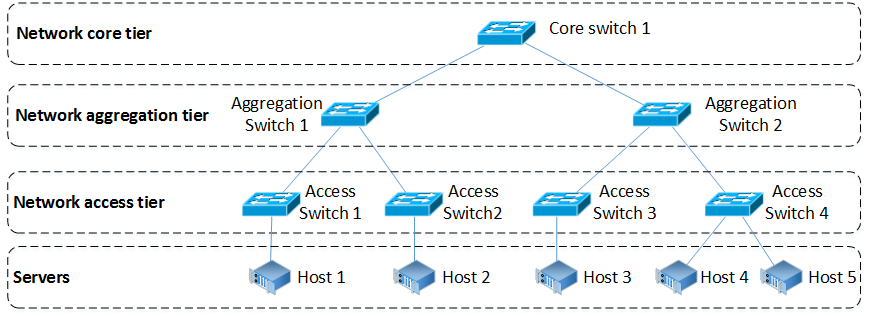
\includegraphics[scale=0.70]{network_topology}
	\caption{Typical datacenter topology}
	\label{fig:network_topology}
\end{figure}
%
\section{Elastic SDN controller cluster}
\label{section:functional-tests}
The first batch of tests carried out were functional tests, designed to validate the correctness of the implementation and the validity of the architecture.\\
%
For the validation of the \gls{SDN} controller elastic cluster described in Chapter \ref*{chapter:implementation} Section \ref{section:SDN-controller-cluster-implementation}, the correctness of such implementation greatly depended on the correctness of the Floodlight controller, and it is therefore considered that any behavior coherent with that of the base version of Floodlight is therefore correct.
Furthermore, all architecture-specific behavior must be validated with the requirements and desired behavior described in Chapter \ref*{chapter:architecture} Section \ref{section:SDN-controller-cluster}.\\
%
The request router, while partially implemented as stated in Section \ref{section:test-environment}, was also subject to testing to the remaining components that were implemented in the test environment.
The validation of the correctness of the request router is validated with the requirements and desired behavior described in Chapter \ref*{chapter:architecture} Section \ref{section:request-router} and implementation specific particularities indicated in Chapter \ref*{chapter:implementation} Section \ref{section:request-router-implementation}.
%
%
\subsection{Scenarios}
\label{subsection:functional-tests-scenarios}
For the \gls{SDN} controller elastic cluster specific functional tests, the scenarios to be tested are as follows:
\begin{enumerate}
	\item Validate cluster membership behavior, consistency and exchanged messages. To do so the first two controller instances are to be initiated simultaneously and let them form a cluster while monitoring the network for exchanged messages. After convergence has been reached, a third controller instance is to be introduced and let it join the cluster while still monitoring the network for exchanged messages.
	\item Validate \gls{MIB} consistency throughout the cluster and exchanged messages by manipulating the network topology to add, remove and simulate failure of OpenFlow switches and hosts as well as simulate switch management transference between available controller instances by provoking failure of cluster instances. The management network is to be monitored for exchanged messages throughout the tests.
	\item Validate the correct programming of OpenFlow switches. This functionality is to be validated by means of executing the module implemented as described in Chapter \ref*{chapter:implementation} Section \ref{subsection:poc-application} to allow \gls{TCP} connections between Host 1 and Host 3 as well as between Host 4 and Host 5. 
\end{enumerate}
%
For the request router specific functional tests, the key points tested are as follows:
\begin{enumerate}
	\item Validate request router clustering and state replication by having OpenFlow switches establish management connections to to the \gls{IPAddress} of the \gls{SDN} controller cluster and validating that both request router instances have the same connection state information.
	\item Validate that the component developed as described in Chapter \ref*{chapter:implementation} Section \ref{subsection:elastic-cluster-integration-implementation} properly integrates with the \gls{SDN} cluster as well as with \gls{LVS}'s ipvsadm tool by provoking \gls{SDN} controller cluster membership changes.
\end{enumerate}
%
\subsection{Results}
\label{section:functional-tests-results}
%
The results obtained from the execution of the functional tests on the experimental implementation show that the proposed architecture provides the desired properties and moreover that the implementation's behavior is coherent with that of the Floodlight.
Furthermore, the request router also complied with the specifications and expected implementation behavior.\\
%
Through the execution of the functional tests for the \gls{SDN} controller elastic cluster, it was found that all relevant network events such as switch, host, links registration/de-registration as well as inter-switch adjacencies are being correctly and timely detected and properly handled to update the local \gls{MIB} and trigger appropriate messages to peer cluster members, which also update their \gls{MIB} accordingly.
It was also confirmed that all messages described in Table \ref{table:cluster-message-spec} within the scope of cluster membership and targeting the whole cluster are sent using multicast, therefore keeping the desired group communication properties described in Chapter \ref*{chapter:architecture} Section \ref{section:SDN-controller-cluster}.\\
%
The functional tests to which the request router was subjected to were used to validate its correct behavior.
However, these tests also led to the discovery of a Master/Master cluster feature instead of the predicted Master/Slave cluster as per \gls{LVS}'s documentation.
%
\section{Distributed network policy module tests}
\label{section:performance-tests}
The use-case scenario of a global policy application that was previously functionally tested was also subject to performance benchmarking.
To that extent, the same scenario used to validate the correct programming of OpenFlow switches was also used to retrieve latency metrics for the programming process.
%
\subsection{Scenario}
\label{subsection:performance-tests-scenario}
Once again, this scenario specified the correct programming of the OpenFlow switches in order to allow for the establishment of \gls{TCP} connections between Host 1 and Host 3 as well as between Host 4 and Host 5.
To fully test the flow programming capabilities, Flow Entries were configured with matches for \gls{OSI} Layer 2, 3 and 4 source and destination fields as well as \gls{OSI} Layer 4 protocol number and physical port through which the traffic was being admitted into the network, coming to a total of 8 match fields per Flow Entry.\\
Since the tests were performed using \gls{TCP} connections, bi-directionality is implied, which means that for every \gls{TCP} session opened there will be two Flow Entries programmed in each of the involved OpenFlow switches.
For completeness purposes and in order to provide scalability metrics, these tests were performed using a two-instance controller cluster and repeated using a three-instance controller cluster, with OpenFlow switches evenly distributed among them by the request router component.
%
\subsection{Results}
\label{subsection:performance-tests-results}
%
The results obtained are stated in Tables \ref{table:perfomance-tests-2controllers} and \ref{table:perfomance-tests-2controllers} and summarized in Figure \ref{fig:performance}.
%
\begin{figure}
	\centering
	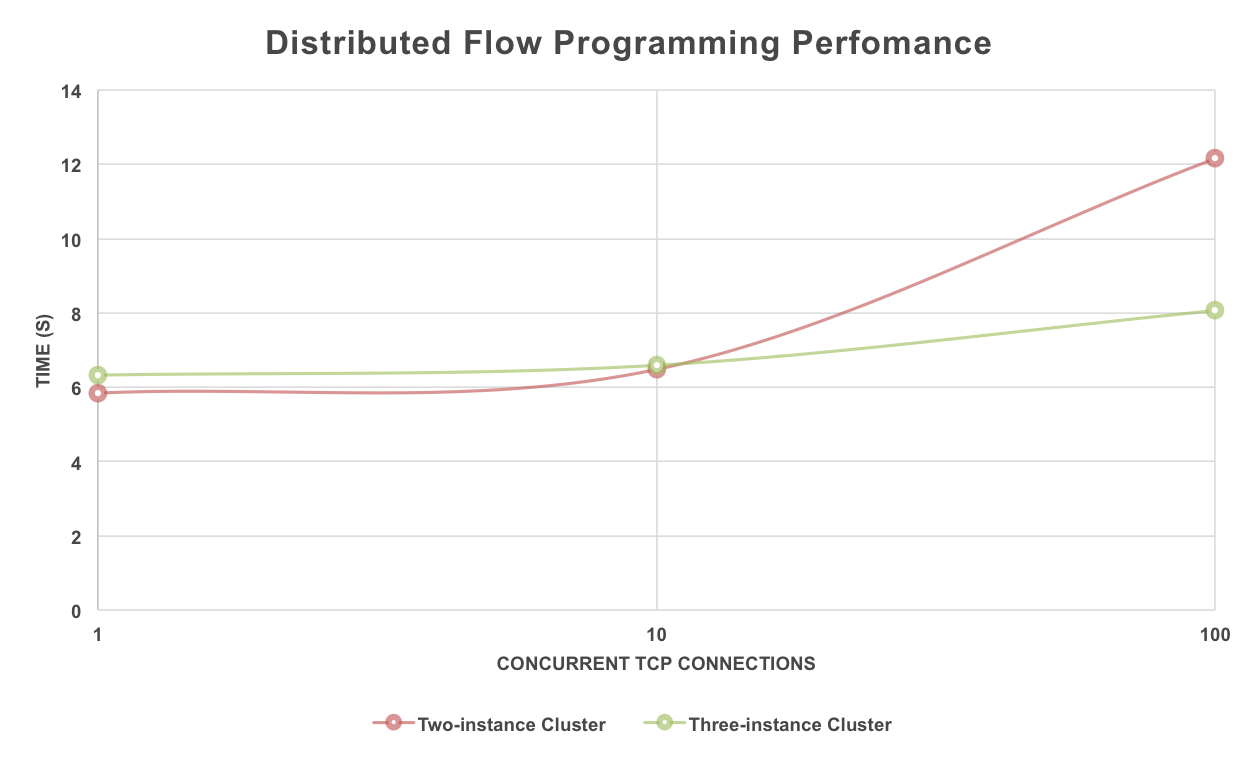
\includegraphics[scale=0.65]{performance_results.png}
	\caption{Performance indicators for the distributed network policy module}
	\label{fig:performance}
\end{figure}
%
\begin{table}[h!]
	\begin{center}
		\rowcolors{2}{EvenRowColor}{OddRowColor}
		\begin{tabular}{ | c | c | c | }
			\rowcolor{HeaderRowColor}
			\hline
			\textbf{1 connection} & \textbf{5 Simultaneous connections} & \textbf{10 Simultaneous connections}\\
			\hline
			6207 milliseconds & 6618 milliseconds & 11714 milliseconds \\
			\hline
			6209 milliseconds & 6414 milliseconds & 14918 milliseconds \\
			\hline
			4406 milliseconds & 6614 milliseconds & 11270 milliseconds \\
			\hline
			4406 milliseconds & 6410 milliseconds & 11709 milliseconds \\
			\hline
			6406 milliseconds & 6609 milliseconds & 14919 milliseconds \\
			\hline
			6406 milliseconds & 6414 milliseconds & 11705 milliseconds \\
			\hline
			6406 milliseconds & 6413 milliseconds & 10725 milliseconds \\
			\hline
			6006 milliseconds & 6213 milliseconds & 10738 milliseconds \\
			\hline
			6206 milliseconds & 6609 milliseconds & 11722 milliseconds \\
			\hline
		\end{tabular}
		\caption{Flow programming results with a two-instance controller cluster}
		\label{table:perfomance-tests-2controllers}
	\end{center}
\end{table}
%
\begin{table}[h!]
	\begin{center}
		\rowcolors{2}{EvenRowColor}{OddRowColor}
		\begin{tabular}{ | c | c | c | }
			\rowcolor{HeaderRowColor}
			\hline
			\textbf{1 connection} & \textbf{5 Simultaneous connections} & \textbf{10 Simultaneous connections}\\
			\hline
			6606 milliseconds & 6614 milliseconds & 6681 milliseconds \\
			\hline
			6406 milliseconds & 6614 milliseconds & 6678 milliseconds \\
			\hline
			6206 milliseconds & 6610 milliseconds & 10686 milliseconds \\
			\hline
			6406 milliseconds & 6614 milliseconds & 6682 milliseconds \\
			\hline
			6206 milliseconds & 6414 milliseconds & 6685 milliseconds \\
			\hline
			6206 milliseconds & 6614 milliseconds & 10686 milliseconds \\
			\hline
			6406 milliseconds & 6618 milliseconds & 6690 milliseconds \\
			\hline
			6406 milliseconds & 6609 milliseconds & 10698 milliseconds \\
			\hline
			6006 milliseconds & 6610 milliseconds & 7092 milliseconds \\
			\hline
		\end{tabular}
		\caption{Flow programming results with a three-instance controller cluster}
		\label{table:perfomance-tests-3controllers}
	\end{center}
\end{table}
%
\section{Analysis}
\label{section:considerations}
Due to Mininet's limitations, switches and hosts cannot be added or removed dynamically, however, they can be isolated from the network by shutting down all ports and in the particular case of switches removing configuration for controller connection.
It is not evident however that this limitation impacted the tests in anyway.\\
%
The results obtained from the tests to the \gls{SDN} controller elastic cluster showed that both cluster membership and \gls{MIB} are kept consistent throughout cluster members after adding, removing and provoking deliberate failures on controller instances as well as OpenFlow switches.\\
While the functional tests to both controller and request router implementations yielded positive results, the results obtained while benchmarking the distributed network policy application are unsatisfactory, which might be related to the overall load of the hardware supporting the test environment and to a poor implementation of \gls{TCP} unicast connections between controller instances, which instead of being cached for further communications are being opened and closed to send a single message. 
It is noticeable however that the addition of more \gls{SDN} controller instances to the cluster and consequent redistribution of the OpenFlow switches between them does not affect the overall time required to execute the distributed flow programming.\\
The global memory footprint of the controller instances appear to have suffered an increase of approximately $10\%$.
 
%!TEX root = ../dissertation.tex

\chapter{Conclusion}
\label{chapter:conclusion}
\gls{SDN} presents itself as the solution for traditional network management problems, and OpenFlow while being the most promising protocol implementing the \gls{SDN} architecture offers two different approaches to program the network, namely reactive and proactive programming.\\
While reactive programming offers a much more flexible and convenient method to program the network, it comes with a computational cost that becomes a limitation when applied to large scale networks.\\
In this work we proposed a novel architecture for OpenFlow controllers based on the concept of SDN controller elastic clustering and coupled with a load balance infrastructure.
The proposed architecture provides a scalable solution for reactive programming in large networks and, at the same time, increased redundancy and resilience in case of failure of a single controller, while keeping the centralized management paradigm typical to \gls{SDN} and without introducing complex distributed coordination algorithms in the controller implementation.\\
To validate the proposed architecture, we implemented a prototype of the \gls{SDN} controller cluster by extending version 1.1 of the Floodlight controller.
A prototype of the load balance infrastructure was also implemented, using free open-source components such as Quagga and \gls{IPVS} and relaying in proven standards such as \gls{BGP} and \gls{BFD}.\\
%
The global prototype implementation of the proposed architecture showed that it is able to provide a fully functional elastic controller cluster for \gls{SDN} applications, thus removing the limitations of OpenFlow's reactive programming when deployed in large networking environments.\\
%
Along with the implementation of the prototype a sample \gls{SDN} application was also developed in order to demonstrate the use of the architecture.
Tests conducted to this applications showed that when network traffic increases and new \gls{SDN} controller instances are added to the cluster, a performance gain of 33$\%$ is attained, further proving the desired scalability properties of the proposed architecture.\\
%
Although the implementation described in this work served its purpose as a prototype, a more carefully developed solution that goes deeper into the controller core implementation will provide a considerable increase in performance.\\
%
The standardization and extension of the message set exchanged between controller instances pertaining to the same cluster and implementation as an Apllication layer protocol will make way for the existence of controller clusters composed of controller instances implemented in different languages and more fit to handle specific needs.



\bibliographystyle{ieeetr}
\addcontentsline{toc}{chapter}{Bibliography}
\bibliography{bibliography/dissertation}

% Appendix
\appendix
%!TEX root = ../dissertation.tex

% Appendix chapters entry point
% Include the chapters below

%\include{appendix/appendixa}


% Glossary and Acronym List
\if\includeGlossary 1
\printglossary
\fi

% Back Cover
\pagenumbering{gobble}
\NewPage

\end{document}
